\chapter{The setup}

\section{Statement of the problem}     \label{statement}



\begin{figure}
 \centering
  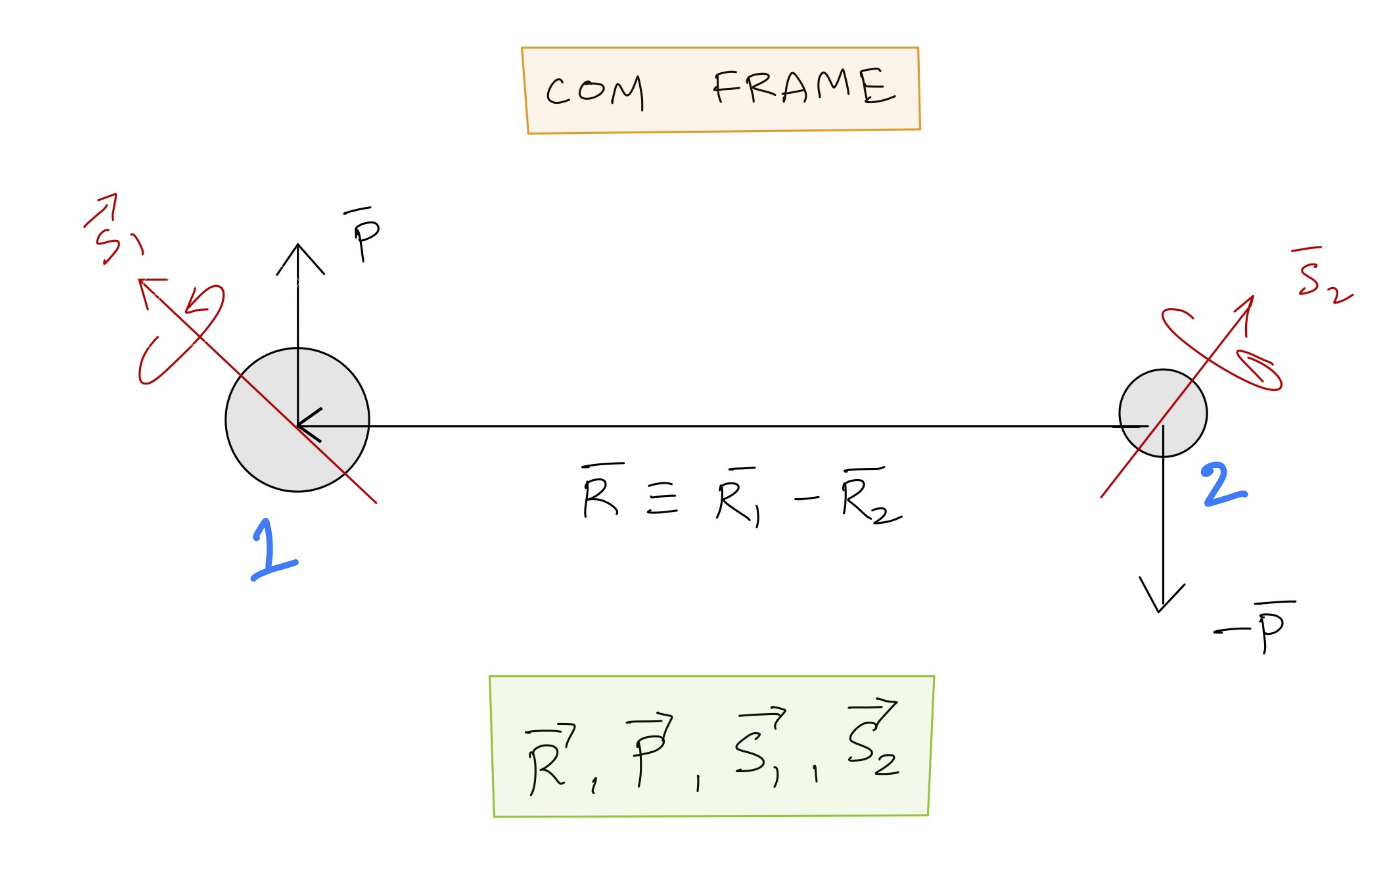
\includegraphics[width=0.9\linewidth]{setup_fig}
  \caption{Schematic setup of a precessing black hole
    binary. All phase space variables are contained in the
    form of four 3D vectors $\vv{R}, \vv{P}, \vv{S}_1$ and $\vv{S}_2$.
    \vspace{-1.em}
  }
  \label{fig:SetupFig}
\end{figure}


We start by describing the canonical variables and the dynamical
setup used to study eccentric binaries of black holes with precessing
spins in the post-Newtonian (PN) approximation. 
The BBH system under consideration is
schematically displayed in Fig.~\ref{fig:SetupFig}, using its
center-of-mass frame \cite{Damour:1988mr}, to define the separation
vector $\vec{R} \equiv \vec{R}_1 -\vec {R}_2$ and the linear momenta
$\vec{P} \equiv \vec{P}_1 = - \vec{P}_2$ of a binary of black holes
with masses $m_1$ and $m_2$. With these quantities, we build the
Newtonian orbital angular momentum $ \vec{L} \equiv \vec{R} \times \vec{P }$,
and the total angular momentum
$\vec{J} \equiv \vec{L} + \vec{S}_{1}+ \vec{S}_{2}$ which includes the BH
spins $\vec{S}_{1}$ and $ \vec{S}_{2}$. The individual BH masses are
$m_1$ and $m_2$ and the total mass $M \equiv m_1+m_2 $.
Additionally, the reduced mass is given by $\mu\equiv m_1m_2/M$ and the symmetric
mass ratio $\nu\equiv\mu/M$ is a function of the reduced mass.
The constants $\sigma_1 \equiv 1 + 3 m_{2}/4 m_{1}$ and
$\sigma_2 \equiv 1 + 3 m_{1}/4 m_{2}$ are used to build the effective
spin
\begin{equation}
  \vec{S}_{\mathrm{eff}} \equiv  \sigma_1 \vec{S}_{1} + \sigma_2\vec{S}_2 \,.
  \label{eq:seff}
\end{equation}

In terms of the scaled variables $\vec{r} \equiv \vec{R} / G M, \vec{p} \equiv \vec{P} / \mu$,
the 1.5 post-Newtonian (PN) Hamiltonian is given by 
\cite{Barker:1966zz, Damour:2001tu,
  Barker:1975ae, Hartl:2004xr,Steinhoff:2010zz}
\begin{align}
  H  =  H_{\mathrm{N}}   +    H_{1\mathrm{PN}}  +    H_{1.5\mathrm{PN}}   + \mathcal{O}(c^{-4})
  \,,
  \label{Hamiltonian-1}
  \end{align}
 where 
\begingroup
\allowdisplaybreaks
\begin{align}
H_{\mathrm{N}}       ={} &   \mu\left(\frac{p^2}{2}     -    \frac{1}{r}\right)  ,      \label{eq:int1a}    \\
H_{\mathrm{1PN}}     ={} &   \frac{\mu}{c^2}\bigg\{  \frac{1}{8}(3 \nu-1) p^4     +  \frac{1}{2r^2}       \nonumber  \\
   &   - \frac{1}{2 r}  \left[   (3+ \nu) p^2  +  \nu (\hat{r}\cdot \vec{p})^2  \right]\bigg\}    ,        \\
H_{\mathrm{1.5PN}}   ={} &   \frac{ 2 G }{c^{2} R^{3}} \SeffL   ,             \displaybreak[0]
   \,.
\label{Hamiltonian-2}
\end{align}
\endgroup



\textbf{The problem:} The above 1.5PN Hamiltonian is  a function of the 
phase-space variables $\vec{R}(t), \vec{P}(t), \vec{S}_1(t)$ and $\vec{S}_2(t) $
only. Our challenge is to integrate the Hamilton's equations
obtained from this Hamiltonian to obtain the solution $\vec{R}(t),
 \vec{P}(t), \vec{S}_1(t)$ and $\vec{S}_2(t) $. This is the subject of these 
 lecture notes.




\section{Defining the 1.5PN BBH system}        \label{defining the system}


In graduate level classical mechanics, specification of the Hamiltonian 
$H( \vv{p}, \vv{q})$ is considered equivalent to specifying the system, for 
the application of Hamiltons's equations  \cite{goldstein2013classical}
\begin{align}    \label{Hamilton's_eqns}
\dot{q_i} =  \frac{\partial H}{\partial p_i},~  ~~~~~~~~~~~~~
\dot{p_i} = - \frac{\partial H}{\partial q_i},
\end{align}
immediately furnishes the equations 
of motion (EOMs). Eqs.~\eqref{Hamilton's_eqns} further imply  that
any function $f(p,q)$ of the phase space variables obeys (Eq. 9.94 of
Ref.~\cite{goldstein2013classical})
\begin{align}    
\frac{d f}{d t}   & = \pb{f, H} + \frac{\partial f}{\partial t} = \pb{f, H}, ~~~~~~~~~~~~~~~~\text{where}    \label{EOM-PB}  \\
\{f, g\} &\equiv  \sum_{i=1}^{N}\left(\frac{\partial f}{\partial q_{i}} \frac{\partial g}{\partial p_{i}}-\frac{\partial f}{\partial p_{i}} \frac{\partial g}{\partial q_{i}}\right)    \label{PB_defined}
\end{align}
where the last equality in Eq.~\eqref{EOM-PB}
 is valid if the Hamiltonian $H$ is not a 
function of time (which will be the case for our BBH system, the subject of
these lecture notes). $\pb{f,g}$ is called the Poisson bracket (PB)
between $f$ and $g$. Actually,
\begin{center}
Eq.~\eqref{Hamilton's_eqns}    $\Leftrightarrow$   Eq.~\eqref{EOM-PB},
\end{center}
i.e., the implication goes both ways; the two equations are equivalent.




Our point of view towards the PB-based EOMs for these lecture notes will be somewhat 
different from the above standard approach adopted by classical mechanics texts. 
For the BBH system with 
phase-space variables $\vec{R}(t), \vec{P}(t), \vec{S}_1(t)$ and $\vec{S}_2(t) $,
the EOMs for any general function 
$f(\vec{R}(t), \vec{P}(t), \vec{S}_1(t),\vec{S}_2(t))$ is still given by
Eq.~\eqref{EOM-PB}.   
But instead of Eq.~\eqref{PB_defined}, we define the PBs via
\begin{align}     \label{PBs_defined_1}
\left\{R_{i}, P_{j}\right\}=\delta_{{j}{i}} \quad \text { and } \quad\left\{S_{A}^{i}, S_{B}^{j}\right\}=\delta_{A B} \epsilon_{k}^{i j} S_{A}^{k}, 
\end{align}      
where the labels $A$ and $B$ refer to the two BHs. How to
define the PB between any two functions $f$ and $g$ 
of the phase-space variables? We simply axiomatize the anti-commutativity,
bilinearity, product,
and the chain rules for the PBs
\begin{subequations}     \label{PBs_defined_2}
\begin{equation}
\pb{f,g}   =  - \pb{g,f}   ,   
\end{equation}
\begin{equation}
\{a f+b g, h\}=a\{f, h\}+b\{g, h\}, \quad\{h, a f+b g\}=a\{h, f\}+b\{h, g\}, \quad a, b \in \mathbb{R}    ,  
\end{equation}
\begin{equation}
\{f g, h\}=\{f, h\} g+f\{g, h\}  ,
\end{equation}
 \begin{equation}
\pb{f, g (v_i)}  =  \pb{f, v_i}  \frac{\pd g}{\pd v_i}   ,  
\end{equation}
\end{subequations}
where $v_i$ represents any of the phase-space variables.
The PB between any two phase space variables, i.e. components of
$\vec{R}(t), \vec{P}(t), \vec{S}_1(t)$ and $\vec{S}_2(t) $ which 
does not fall under the purview of
 Eqs.~\eqref{PBs_defined_1} and \eqref{PBs_defined_2} is assumed to vanish.
 Note that Eq.~\eqref{PB_defined} implies Eqs.~\eqref{PBs_defined_2}, 
 but for these lecture notes,
  we will take the latter as definitions and totally disregard 
 the former.



We therefore have defined our system of interest completely in that 
we can now write its EOM. This definition consists of
\begin{itemize}
\item specifying the Hamiltonian via Eq.~\eqref{Hamiltonian-1}.
\item axiomatizing Eqs.~\eqref{PBs_defined_1}, and \eqref{PBs_defined_2}.
 These enable us to evaluate the PB between any 
two functions of the phase-space variables.
\item stating the EOM via Eq.~\eqref{EOM-PB}.
\end{itemize}
Note that in this slightly different point of view,
we don't try to define the PBs via partial derivatives 
as in Eq.~\eqref{PB_defined}. Also, note that it appears as if there is no way
to recover the spin PB of Eq.~\eqref{PBs_defined_1} via Eq.~\eqref{PB_defined}.
In this sense, this new way of defining the PB seems more general.





\begin{Exercise}    \label{exercise-1}
\textbf{Problem:} Compute the PB 
\begin{align}
\pb{R_x , \sin  P_x   +   P_x  }.
\end{align}

\textbf{Solution:} 
\begin{align}
& \pb{R_x , \sin  P_x   +   P_x  }  ,   \\ 
& =  \pb{R_x,  \sin  P_x  }  +  \pb{R_x,   P_x  }  ,  \\
& =  \pb{R_x,    P_x  }  \frac{\pd \sin P_x}{\pd P_x}  +  \pb{R_x,   P_x  }  ,  \\
&  =   \cos P_x + 1.
\end{align}
Use has been made of the second and the fourth of Eqs.~\eqref{PBs_defined_2}
in the above manipulations.
\end{Exercise}


We have prepared a
\textsc{Mathematica} package \cite{MMA1}
which can compute the PB between any two quantities,
based on the PB theory discussed above.




If we try to compute the PB between the azimuthal angle 
$\phi_{A} = \arctan (S_A^y/S_A^x)$ of the spin vector
of a BH and its $z$-component, it can be checked (using 
Eqs.~\eqref{PBs_defined_1} and \eqref{PBs_defined_2}) that it comes out to be
\begin{equation}
\left\{\phi_{A}, S_{B}^{z}\right\}=\delta_{A B}  ,     \label{spin-PB}
\end{equation}
which upon comparison with Eqs.~\eqref{PBs_defined_1}
makes us conclude that $\phi_A$ and $S_{A}^{z}$ respectively ``act
like'' position and momentum variables respectively. This is of big significance 
when we deal with the action-angle variables (AAVs) later. AAVs are the key
to obtaining the closed-form solutions we have set out to seek. 
We end this section 
with a definition. \\ \\
\textbf{Commuting quantities: } Two quantities {commute} if their PB vanishes.


